\documentclass{article}
\usepackage[utf8]{inputenc}
\usepackage{amsmath}
\usepackage{amssymb}
\usepackage{multicol}
\usepackage{geometry}
\usepackage{float}
\usepackage{hyperref}
\usepackage{caption}
\usepackage{subcaption}
\usepackage{graphicx}
\usepackage{expl3}
\usepackage{xparse}
\usepackage{array}
\usepackage{booktabs}
\usepackage{tabularx}
\usepackage[table, svgnames]{xcolor}
\usepackage{csquotes}
\usepackage{titling}
\usepackage{enumitem}
\usepackage{comment}
\usepackage{lipsum}
\usepackage{bm}
\usepackage{mathtools}

% https://answerbun.com/
% https://tex.stackexchange.com/questions/88929/vertical-table-lines-are-discontinuous-with-booktabs

\setlength{\droptitle}{-5em} %-5em
\geometry{left=1cm,right=1cm,top=2cm,bottom=2cm}
\graphicspath{{images/}}
\captionsetup[table]{skip=5pt}

\hypersetup{
    pdftitle={Parallelization of the SLINK clustering algorithm},
    pdfauthor={Alessio De Biasi (870288); Jonathan Gobbo (870506)},
    hidelinks,
    pdfcreator={XeLaTeX}}

\title{Parallelization of the SLINK clustering algorithm\vspace{-1.25ex}}
\author{Alessio De Biasi (870288) \and Jonathan Gobbo (870506)}
\date{August 2022}

% Options for packages loaded elsewhere
\PassOptionsToPackage{unicode}{hyperref}
\PassOptionsToPackage{hyphens}{url}

\newenvironment{tablelayout}[1][]{
    \begin{table}[H]
        \centering
        \caption{#1}
        \begin{tabular}[H]{ccccccc}
            \hline
            & s1 & s2 & s3 & s4 & tot & \\
            \hline
            }{
            \\
            \hline
        \end{tabular}
        \label{tab:my_label}
    \end{table}
}

\newenvironment{tablelayout2}{
    \begin{table}[H]
        \centering
        \begin{tabular}[H]{lrrrrrr}
            \hline
            DS & \centering s1 & \centering s2 & \centering s3 & s4 & s5 & tot \\
            \hline
            }{
            \\
            \hline
        \end{tabular}
        \label{tab:my_label}
    \end{table}
}

\ExplSyntaxOn
\NewDocumentCommand{\formatNumber}{mm} {
\seq_set_split:Nnn \values {.} {#1}
\seq_item:Nn \values {1}
\int_compare:nNnTF{\seq_count:N \values} = {2}
    {.\footnotesize    \seq_item:Nn \values {2}}
    {}
\normalsize$\,$#2
}
\NewDocumentEnvironment{tableLayout}{mb}{
\setlength\intextsep{2mm}
\renewcommand{\divisor}{\midrule}
\seq_set_split:Nnn \l_rows_seq { \\ } {#2}
\begin{table}[H]
\centering
\begin{tabularx}{0.98\linewidth}[H]{
>{\raggedright}p{1.8em}|
%!{\color{Gainsboro!50!Lavender}\vline width 0.75em}
>{\raggedleft}X
>{\raggedleft}X
>{\raggedleft}X
>{\raggedleft}X
>{\raggedleft\arraybackslash}X
}
\toprule
\textbf{DS} &
\multicolumn{1}{c}{\hspace{1.2em}\textbf{S1}} &
\multicolumn{1}{c}{\textbf{S2}} &
\multicolumn{1}{c}{\textbf{S3}} &
\multicolumn{1}{c}{\textbf{S4}} &
\multicolumn{1}{c}{\textbf{Total}} \\
\toprule
\seq_use:Nn \l_rows_seq {\\}\\
\bottomrule
\end{tabularx}
\caption{#1}
\end{table}
}{}

\NewDocumentEnvironment{tableLayout2}{mb}{
\setlength\intextsep{2mm}
\renewcommand{\divisor}{\midrule}
\seq_set_split:Nnn \l_rows_seq { \\ } {#2}
\begin{table}[H]
\centering
\begin{tabularx}{0.98\linewidth}[H]{
>{\raggedright}p{1.8em}|
%!{\color{Gainsboro!50!Lavender}\vline width 0.75em}
>{\raggedleft}p{1.8em}
>{\raggedleft}X
>{\raggedleft}X
>{\raggedleft}X
>{\raggedleft}X
>{\raggedleft\arraybackslash}p{3.2em}
}
\toprule
\textbf{DS} &
\multicolumn{1}{c}{\hspace{0.4em}\textbf{S1}} &
\multicolumn{1}{c}{\textbf{S2}} &
\multicolumn{1}{c}{\textbf{S3}} &
\multicolumn{1}{c}{\textbf{S4}} &
\multicolumn{1}{c}{\textbf{S5}} &
\multicolumn{1}{c}{\textbf{Total}} \\
\toprule
\seq_use:Nn \l_rows_seq {\\}\\
\bottomrule
\end{tabularx}
\caption{#1}
\end{table}
}{}
\ExplSyntaxOff

\newcommand{\divisor}{& \\[-2.25ex]\hline& \\[-2.25ex]}
\newcommand{\s}{$\,$s}
\newcommand{\ms}{$\,$ms}
\newcommand{\m}{$\,$m$\ $}

\setlength{\itemsep}{0pt}
\setlength{\parskip}{0pt}
\setlist{itemsep=0.25mm,
% Margin of the whole list
topsep=0.25mm,
% Padding between each element of the list
parsep=0.25mm}

\begin{document}
\twocolumn
\maketitle

\section{Introduction}

The purpose of this project is to implement the SLINK clustering algorithm and to apply
parallelization techniques to improve its performance.

All the implementations of the clustering algorithms are written in \texttt{C++20} and they are
compiled with the GCC G++ 12.1.1 (Red Hat) compiler, using the \texttt{-O3} and
\texttt{-march=native} flags.

In particular, we tested the clustering algorithm implementations on two datasets:
\begin{itemize}
\item Accelerometer\footnote{https://archive.ics.uci.edu/ml/datasets/Accelerometer} (A), composed
of 153'000 samples, each of which with 5 attributes. For the tests we have performed, we have
selected only the last 3 of them;
\item Generated (G), composed of 100'000 samples, each of which with 45 randomly generated real
attributes uniformly distributed in the range 0-100.
\end{itemize}

We will report the mean execution time of 3 executions of each implementation on the two datasets,
run on a machine equipped with an AMD Ryzen 7 1700 CPU with 8 cores and 16 threads, 16 GB of RAM,
and running Fedora Workstation 36.
In particular, we measured the time taken by each step of the pseudo-code (reported as S1, S2, S3
and S4) to be executed.

In all the tests we used a \texttt{std::vector} to hold the values of $\pi$ and $\lambda$.

Note that the reported total times include also some extra time spent by the various
implementations to perform operations like allocating and de-allocating the memory, or copying
the iterators.

Moreover, for space reasons, in some tests we do not report the results obtained using 2 and 16
threads

\hypertarget{implementations}{
\section{Implementations}
\label{implementations}}

\hypertarget{sequential}{
\subsection{Sequential}
\label{sequential}}

We first implemented the sequential version of the clustering algorithm.
This implementation is just the translation in \texttt{C++} code of the pseudo-code reported in
the slides.

Data is supplied as a
\texttt{std::vector\textless{}double\ *\textgreater{}}, i.e., a vector
of pointers to heap-allocated arrays, where each of these arrays holds the attributes of one data
sample.

\begin{tableLayout}{Execution times of the sequential implementation}
A & 19\ms & 1\m 30\s & \formatNumber{37.330}{s} & \formatNumber{20.271}{s} & 2\m 28\s \\
\divisor
G & 19\ms & 8\m 59\s & \formatNumber{16.246}{s} & \formatNumber{12.802}{s} & 9\m 28\s
\end{tableLayout}


\hypertarget{parallel-distance}{%
\subsection{Multithreaded distance computation}\label{parallel-distance}}

From the previous tests results, we saw that he computation of the distances is the step of the
algorithm taking most of the time to be executed.

Since each distance can be computed independently from the others, their computation can be
easily made parallel by using the \emph{OpenMP} library.

The supplied data has the same memory layout as before.

\begin{tableLayout}{Execution times of the first parallel implementation}
A2 & 10\ms & \formatNumber{43.043}{s} & \formatNumber{39.568}{s} & \formatNumber{23.286}{s} & 1\m
46\s \\
A4 & 11\ms & \formatNumber{29.641}{s} & \formatNumber{36.144}{s} & \formatNumber{23.609}{s} & 1\m
29\s \\
A8 & 11\ms & \formatNumber{20.940}{s} & \formatNumber{35.260}{s} & \formatNumber{23.541}{s} & 1\m
20\s \\
A12 & 10\ms & \formatNumber{24.402}{s} & \formatNumber{36.713}{s} & \formatNumber{24.204}{s} &
1\m 25s \\
A16 & 11\ms & \formatNumber{27.201}{s} & \formatNumber{47.172}{s} & \formatNumber{26.257}{s} &
1\m 41\s \\
\divisor
G2 & 13\ms & 4\m 12\s & \formatNumber{15.228}{s} & \formatNumber{13.855}{s} & 4\m 41\s \\
G4 & 15\ms & 2\m 23\s & \formatNumber{15.555}{s} & \formatNumber{14.881}{s} & 2\m 53\s \\
G8 & 14\ms & 1\m 34\s & \formatNumber{15.305}{s} & \formatNumber{14.977}{s} & 2\m 04\s \\
G12 & 12\ms & 1\m 43\s & \formatNumber{17.569}{s} & \formatNumber{15.308}{s} & 2\m 16\s \\
G16 & 12\ms & 1\m 42\s & \formatNumber{20.592}{s} & \formatNumber{15.668}{s} & 2\m 18\s
\end{tableLayout}

\hypertarget{parallel-sse-avx}{%
\subsection{SSE and AVX in the computation of the distances}\label{parallel-sse-avx}}

Since the attributes of the data samples to cluster are stored contiguously in memory, we decided
to improve the previous solution using the SSE and AVX instructions when computing the distances.

Indeed, to compute the distance between two points, the algorithm perform the same instructions
(difference and square) to every pair of attributes.

\begin{tableLayout}{Execution times of the implementation using SSE}
A2 & 11\ms & \formatNumber{46.922}{s} & \formatNumber{32.362}{s} & \formatNumber{21.116}{s} & 1\m
40\s \\
A4 & 11\ms & \formatNumber{34.329}{s} & \formatNumber{35.250}{s} & \formatNumber{23.791}{s} & 1\m
33\s \\
A8 & 9\ms & \formatNumber{27.252}{s} & \formatNumber{35.007}{s} & \formatNumber{23.633}{s} & 1\m
26\s \\
A12 & 10\ms & \formatNumber{27.328}{s} & \formatNumber{37.252}{s} & \formatNumber{24.346}{s} &
1\m 29\s \\
A16 & 12\ms & \formatNumber{28.596}{s} & \formatNumber{47.285}{s} & \formatNumber{26.313}{s} &
1\m 42\s \\
\divisor
G2 & 14\ms & 4\m 29\s & \formatNumber{16.732}{s} & \formatNumber{14.733}{s} & 5\m 00\s \\
G4 & 15\ms & 2\m 33\s & \formatNumber{19.175}{s} & \formatNumber{16.085}{s} & 3\m 08\s \\
G8 & 13\ms & 1\m 39\s & \formatNumber{19.319}{s} & \formatNumber{15.894}{s} & 2\m 15\s \\
G12 & 13\ms & 1\m 43\s & \formatNumber{18.766}{s} & \formatNumber{15.457}{s} & 2\m 18\s \\
G16 & 14\ms & 1\m 39\s & \formatNumber{21.918}{s} & \formatNumber{15.986}{s} & 2\m 17\s
\end{tableLayout}

\begin{tableLayout}{Execution times of the implementation using AVX}
A2 & 8\ms & \formatNumber{39.106}{s} & \formatNumber{38.321}{s} & \formatNumber{23.127}{s} & 1\m
41\s \\
A4 & 10\ms & \formatNumber{24.656}{s} & \formatNumber{37.981}{s} & \formatNumber{23.659}{s} & 1\m
26\s \\
A8 & 8\ms & \formatNumber{17.814}{s} & \formatNumber{37.826}{s} & \formatNumber{23.772}{s} & 1\m
19\s \\
A12 & 8\ms & \formatNumber{18.416}{s} & \formatNumber{40.067}{s} & \formatNumber{24.198}{s} & 1\m
23\s \\
A16 & 10\ms & \formatNumber{19.824}{s} & \formatNumber{52.452}{s} & \formatNumber{26.367}{s} &
1\m 39\s \\
\divisor
G2 & 13\ms & 4\m 34\s & \formatNumber{14.860}{s} & \formatNumber{14.236}{s} & 5\m 03\s \\
G4 & 15\ms & 2\m 37\s & \formatNumber{15.111}{s} & \formatNumber{15.457}{s} & 3\m 07\s \\
G8 & 14\ms & 1\m 42\s & \formatNumber{15.143}{s} & \formatNumber{15.660}{s} & 2\m 13\s  \\
G12 & 14\ms & 1\m 49\s & \formatNumber{17.418}{s} & \formatNumber{15.516}{s} & 2\m 22\s \\
G16 & 14\ms & 1\m 44\s & \formatNumber{20.112}{s} & \formatNumber{15.970}{s} & 2\m 20\s
\end{tableLayout}

We expected this implementation to work faster than the previous one but, as the results show,
this implementation works slightly slower than the previous one.

Investigating using the \textit{perf} tool, we discovered that most of the time the CPU is
stalled due to a high rate of cache misses (about 80\% of all the data memory accesses).

\hypertarget{a-new-data-structure}{%
\subsection{A new data structure}\label{a-new-data-structure}}

Therefore, we decided to change the data structure holding the data samples to cluster in flavour
to a more a contiguous one.

In particular, we chose to organize the data as a unique heap-allocated array, where the data
samples are stored one after the other, like the attributes of each sample.

\begin{tableLayout}{Execution times of the implementation using a contiguous data structure and
SSE (2 and 16 threads tests omitted)}
A4 & 4\ms & \formatNumber{11.770}{s} & \formatNumber{34.453}{s} & \formatNumber{23.509}{s} & 1\m
10\s \\
A8 & 4\ms & \formatNumber{7.531}{s} & \formatNumber{35.604}{s} & \formatNumber{23.674}{s} & 1\m
07\s \\
A12 & 4\ms & \formatNumber{8.277}{s} & \formatNumber{37.068}{s} & \formatNumber{24.300}{s} & 1\m
10\s \\
\divisor
G4 & 9\ms & \formatNumber{44.391}{s} & \formatNumber{14.319}{s} & \formatNumber{15.880}{s} & 1\m
15\s \\
G8 & 8\ms & \formatNumber{37.005}{s} & \formatNumber{14.162}{s} & \formatNumber{15.937}{s} & 1\m
07\s \\
G12 & 8\ms & \formatNumber{37.132}{s} & \formatNumber{15.271}{s} & \formatNumber{15.902}{s} & 1\m
08\s
\end{tableLayout}

\begin{tableLayout}{Execution times of the implementation using a contiguous data structure and
AVX(2 and 16 threads tests omitted)}
A4 & 4\ms & \formatNumber{12.462}{s} & \formatNumber{42.709}{s} & \formatNumber{23.633}{s} & 1\m
18\s \\
A8 & 4\ms & \formatNumber{8.315}{s} & \formatNumber{42.649}{s} & \formatNumber{23.517}{s} & 1\m
14\s \\
A12 & 4\ms & \formatNumber{8.368}{s} & \formatNumber{42.744}{s} & \formatNumber{23.809}{s} & 1\m
15\s \\
\divisor
G4 & 10\ms & \formatNumber{46.830}{s} & \formatNumber{14.452}{s} & \formatNumber{15.770}{s} & 1\m
17\s \\
G8 & 8\ms & \formatNumber{38.992}{s} & \formatNumber{14.454}{s} & \formatNumber{16.222}{s} & 1\m
10\s \\
G12 & 8\ms & \formatNumber{39.331}{s} & \formatNumber{15.580}{s} & \formatNumber{15.969}{s} & 1\m
11\s
\end{tableLayout}

As we can see form these results, making the data samples contiguous in memory improves
significantly the performance of the algorithm.

Indeed, when a thread loads 2 or 4 data samples into the extended registers, it is very likely
that another thread has brought them in the L2 cache when requesting the attributes of one of the
data samples stored immediately before in memory.

\hypertarget{stage-3-parallel}{
\subsection{Make the insertion of a new point parallel}
\label{stage-3-parallel}}

After having made parallel the computation of the distances, we focused on making parallel the other
step of the algorithm takes most of the time to complete, i.e., the insertion of a new point to
the dendrogram (i.e., the step \textit{3} of the pseudo-code).

However, there is no chance to make it parallel because, when the element at index $i$ is
analyzed, the algorithm requires that all the elements before have already been analyzed.

Therefore, if we give each thread an element to analyze in a round-robin fashion, then there will
be always a thread working while all the other threads will be blocked waiting for the active
thread to complete its work.

\hypertarget{stage-4-parallel}{
\subsection{Make the rearrangement of the structure of the dendrogram parallel}
\label{stage-4-parallel}}

Therefore, we decided to try to make parallel the third step of the algorithm that takes a
significant amount of time to be executed, i.e., the rearrangement of the structure of the
dendrogram after a new point has been added (i.e., the step \textit{4} of the pseudo-code).

Since each iteration of the \texttt{for} loop is independent from the others, making it parallel
it is almost trivial by using the \emph{OpenMP} library.

Like the last implementation, data is supplied as a unique heap-allocated array.

\begin{tableLayout}{Execution times of the implementation executing in parallel the computation
of the distance (using threads and AVX instructions) as well as the rearrangement of the
structure of the dendrogram}
A4 & 4\ms & \formatNumber{10.599}{s} & \formatNumber{42.538}{s} & \formatNumber{8.939}{s} & 1\m
02\s \\
A8 & 4\ms & \formatNumber{5.836}{s} & \formatNumber{43.255}{s} & \formatNumber{5.659}{s} &
\formatNumber{54.760}{s} \\
A12 & 4\ms & \formatNumber{6.895}{s} & \formatNumber{45.326}{s} & \formatNumber{4.489}{s} &
\formatNumber{56.720}{s} \\
\divisor
G4 & 9\ms & \formatNumber{46.341}{s} & \formatNumber{15.961}{s} & \formatNumber{6.888}{s} & 1\m
09\s \\
G8 & 8\ms & \formatNumber{38.337}{s} & \formatNumber{16.110}{s} & \formatNumber{3.792}{s} &
\formatNumber{58.254}{s} \\
G12 & 8\ms & \formatNumber{39.039}{s} & \formatNumber{17.603}{s} & \formatNumber{3.408}{s} & 1\m
00\s
\end{tableLayout}
For space reasons, we ommitted the results of the implementation when using SSE, since its
execution times that are slightly bigger than the ones of AVX.

\hypertarget{failed-attempt}{
\subsection{A faulty attempt to devise a new algorithm}
\label{failed-attempt}}

The last step of the algorithm we can parallelize is the initialization one (i.e., the step
\textit{1} of the psudo-code). However, as shown by the results, leaving it as-it-is impacts on
the total execution time just for few milliseconds, so trying to making it parallel will likely
not improve the performance of the algorithm any further.

\begin{comment}


To overcome the impossibility of parallelize the step \textit{3} of the algorithm, we decided to
devise a new algorithm, which can be made parallel more easily.

This new algorithm builds incrementally the dendrogram like the algorithm we used so far, but it
is based on a different but simple idea.

Suppose the algorithm needs to add to the dendrogram a new data sample $d$ and suppose that, among
all the samples already added to the dendrogram, the data sample $c$ is the closest one with
distance $l$ (i.e., $c$ is the data sample with the minimum distance from $d$).

Then, any cluster containing $d$ for sure contains also $c$, otherwise there would be another
data sample $e$ already added to the dendrogram which is closer to $d$ more than $c$, but we assumed
$c$ is the closest one.

If we look at the structure of the dendrogram, this consideration implies that the new data sample
$d$ is connected to one of the edges in the path from $c$ to the root of the dendrogram.

\begin{figure}[H]
\centering
\begin{subfigure}{.5\linewidth}
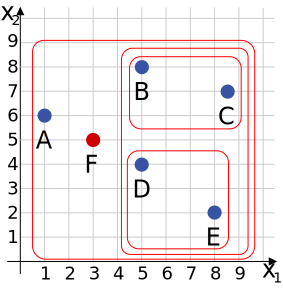
\includegraphics[width=\linewidth]{graph-2}
\caption{Graph with all the points, $F$ is the next point to add}
\end{subfigure}%
\begin{subfigure}{.5\linewidth}
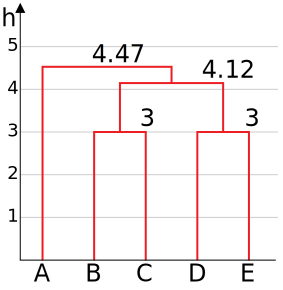
\includegraphics[width=\linewidth]{dendrogram-2}
\caption{Dendrogram}
\end{subfigure}
\caption{Situation}
\end{figure}

In particular, the new edge will be added on that path right before the first edge $\varepsilon$
with an
height that is bigger than $l$.

Therefore, adding a new edge to the dendrogram is trivial if we represent the dendrogram as a
binary tree, where:
\begin{itemize}
\item Each leaf stores the identifier of the data sample and a pointer to the parent node;
\item Each internal node stores the pointer to the parent node and the children nodes, as
well as the value of height of the edge.
\end{itemize}
Indeed, it is just a matter of changing the values of two pointers, namely the pointer to the
left or right child of the node representing the edge $\varepsilon$, and the pointer to the
parent node of the node that was previously connected to $\varepsilon$.

However, this is only half of the work. Suppose, at some point, the cluster $X$ joins cluster $Y$
at distance $k$. Suppose that $c$ belongs to $X$ and suppose that $k > l$.

This implies that $X$ must also contain $d$ because, since $c$ belongs to $X$, then one of the
sub-clusters of $X$ containing $c$ must join the data sample $d$, since the distance between $c$
and $d$ is smaller than $k$.

However, if $X$ joined $Y$ at distance $k$ before adding $d$, now that we have added $d$ the two
clusters may have become closer.

If we look at the dendrogram, this may require to change the heights of all the edges in the path
from the newly added edge to the root of the dendrogram.
Note that, in any case, the heights of any of such edges can't get smaller than the heights of
their children.

Therefore, if in the nodes representing the dendrogram we store also the information about which
point of the left sub-tree is the closest to which point of the right sub-tree, then adjusting
the heights stored in such nodes is trivial.

Indeed, suppose that the node stores the information that the two closest data samples are $e$
and $f$. Suppose also that $d$ belongs to a cluster that also contain $e$. Then, to update the
height of the edge we need to to check if the distance between $d$ and $f$ is smaller than the
distance between $e$ and $f$ (which is the current height of the edge). If so, we need to update
the height of the edge as well as the two closest points (which will be $d$ and $f$). Otherwise,
no change is made.

All of these operations can be easily made parallel. We just need to assign to each thread an
node of the path from $c$ to the root of the dendrogram in a round-robin fashion. The given node
can represent:
\begin{enumerate}
\item An edge with height smaller than $l$. In this case, the thread just does nothing and
selects another edge;

\item The first edge in the path with an height larger than $l$. This can be easily tested
by looking at the heights of the two children, if at least one of them is not a leaf. If they
are both a leaves, then the edge receives by the thread IS the first in the path with an
height larger than $l$.

In this case, the thread just changes the values some the pointers,
which can be done safely by using the \textit{Compare And Swap} primitives offered by the CPU.

\item An edge that does not fall in one of the previous cases. Therefore, the thread needs
only to update the height stored in the node and the two closest points, if the newly added
data sample has made two two sub-clusters closer.
\end{enumerate}

This algorithm is extremely parallel because there almost no data dependency among the nodes the
threads analyze.

However, there are some cases in which this algorithm does not work. Let's take the following
example:

\begin{figure}[H]
\centering
\begin{subfigure}{.5\linewidth}
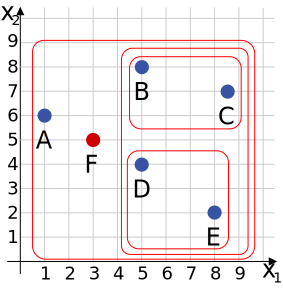
\includegraphics[width=\linewidth]{graph-2}
\caption{Graph with all the points, $F$ is the next point to add}
\end{subfigure}%
\begin{subfigure}{.5\linewidth}
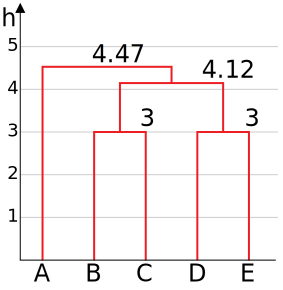
\includegraphics[width=\linewidth]{dendrogram-2}
\caption{Dendrogram}
\end{subfigure}
\caption{Situation}
\end{figure}

When we add to the the dendrogram the point $F$, its structure completely changes:

\begin{figure}[H]
\centering
\begin{subfigure}{.5\linewidth}
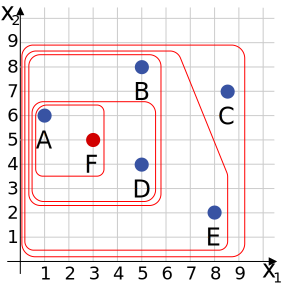
\includegraphics[width=\linewidth]{graph-3}
\caption{Graph with all the points, $F$ is the last added point}
\end{subfigure}%
\begin{subfigure}{.5\linewidth}
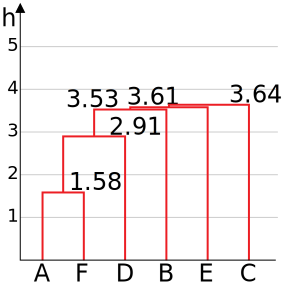
\includegraphics[width=\linewidth]{dendrogram-3}
\caption{Dendrogram}
\end{subfigure}
\caption{Situation}
\end{figure}

This implies that any node of the tree representing the dendrogram can be moved, which implies
that the pointers to the parent and children nodes can change on every node.

Since the threads are traversing the path from a leaf to the root, if a thread moves a node, it
must perform such an operation in mutual exclusion, otherwise the other threads may analyze nodes
that do not belong to the path.

This requires any thread to lock the node they are using, so to prevent any other thread to
traverse the node and analyze the parent of such node, which indeed may change is the thread
moves the node.

All these locks will introduce a high complexity in the algorithm, which leads to poor performances.

Therefore, we abandoned this algorithm, and we tried some micro-optimizations to the algorithm we
have used so far.
\end{comment}

\hypertarget{micro-optimization-partial-sum}{%
\subsection{Partial sums micro-optimization}\label{micro-optimization-partial-sum}}

When the previous implementations use SSE and AVX instructions to compute the distance between
two data samples, they load from memory a bunch of attributes, they compute the pairwise
difference, they square the result and they accumulate it on a stack-allocated variable, which
requires to horizontally sum all the values in the extended registers.
These operations are repeated until no more attributes are left.

The first micro-optimization we have implemented keeps the partial sums of the distances in an
extended register (which acts as the accumulator stack-allocated variable) and performs the
horizontal sum only once, at the end of the computation.

The new implementation combines all the parallelization strategies we have implemented so far
with this micro - optimization.
This implies that the data is still supplied as a unique heap-allocated array.

\begin{tableLayout}{Execution times of the first micro-optimized implementation using AVX (2 and
16 threads tests omitted)}
A4 & 4\ms & \formatNumber{10.174}{s} & \formatNumber{41.862}{s} & \formatNumber{8.887}{s} & 1\m
01\s \\
A8 & 4\ms & \formatNumber{5.820}{s} & \formatNumber{42.804}{s} & \formatNumber{5.592}{s} &
\formatNumber{54.227}{s} \\
A12 & 4\ms & \formatNumber{6.868}{s} & \formatNumber{45.697}{s} & \formatNumber{4.526}{s} &
\formatNumber{57.102}{s} \\
\divisor
G4 & 11\ms & \formatNumber{31.854}{s} & \formatNumber{17.229}{s} & \formatNumber{5.854}{s} & 1\m
05\s \\
G8 & 10\ms & \formatNumber{37.064}{s} & \formatNumber{16.846}{s} & \formatNumber{3.590}{s} &
\formatNumber{57.515}{s} \\
G12 & 9\ms & \formatNumber{37.005}{s} & \formatNumber{17.897}{s} & \formatNumber{3.414}{s} &
\formatNumber{58.330}{s}
\end{tableLayout}

\hypertarget{micro-optimization-no-square-root}{%
\subsection{Square roots micro-optimization}\label{micro-optimization-no-square-root}}

The last micro-optimization we have implemented extends the previous implementation by using the
square of the distances instead of the distances themselves. The computation of the square roots
is applied only at the algorithm and only on the final values of $\lambda$.

Ignoring possible rounding errors, this solution works because the following holds for
non-negative values (as the distances are):
\[
\sqrt{n^2} \geq \sqrt{m^2} \iff n^2 \geq m^2
\]

In the following tables, S5 reports the time taken to compute the square roots.

\begin{tableLayout2}{Execution times of the second micro-optimized implementation using SSE}
A2 & 4\ms & \formatNumber{10.961}{s} & \formatNumber{37.824}{s} & \formatNumber{12.933}{s} &
190$\,\mu$s & 1\m 02\s\\
A4 & 4\ms & \formatNumber{6.641}{s} & \formatNumber{41.826}{s} & \formatNumber{8.989}{s} & 112$\,
\mu$s & \formatNumber{57.466}{s}\\
A8 & 4\ms & \formatNumber{3.903}{s} & \formatNumber{42.693}{s} & \formatNumber{5.592}{s} & 58$\,
\mu$s & \formatNumber{52.199}{s}\\
A12 & 5\ms & \formatNumber{4.603}{s} & \formatNumber{45.701}{s} & \formatNumber{4.549}{s} & 69$\,
\mu$s & \formatNumber{54.864}{s}\\
A16 & 5\ms & \formatNumber{4.067}{s} & \formatNumber{51.38}{s} & \formatNumber{4.222}{s} & 52$\,
\mu$s & \formatNumber{59.340}{s}\\
\divisor
G2 & 9\ms & 1\m 5\s & \formatNumber{15.592}{s} & \formatNumber{9.995}{s} & 113\,$\mu$s & 1\m 30\s\\
G4 & 9\ms & \formatNumber{43.109}{s} & \formatNumber{16.769}{s} & \formatNumber{6.865}{s} & 66$\,
\mu$s & 1\m 07\s\\
G8 & 9\ms & \formatNumber{36.077}{s} & \formatNumber{16.618}{s} & \formatNumber{3.834}{s} & 35$\,
\mu$s & \formatNumber{56.544}{s}\\
G12 & 9\ms & \formatNumber{36.747}{s} & \formatNumber{17.697}{s} & \formatNumber{3.430}{s} &
48$\,\mu$s & \formatNumber{57.890}{s}\\
G16 & 5\ms & \formatNumber{36.383}{s} & \formatNumber{20.554}{s} & \formatNumber{3.100}{s} &
38$\,\mu$s & 1\m 01\s
\end{tableLayout2}

\begin{tableLayout2}{Execution times of the second micro-optimized implementation using AVX}
A2 & 4\ms & \formatNumber{11.439}{s} & \formatNumber{37.881}{s} & \formatNumber{13.146}{s} &
216$\,\mu$s & 1\m 02\s\\
A4 & 4\ms & \formatNumber{7.106}{s} & \formatNumber{42.571}{s} & \formatNumber{8.888}{s} & 115$\,
\mu$s & \formatNumber{58.576}{s}\\
A8 & 4\ms & \formatNumber{4.147}{s} & \formatNumber{42.281}{s} & \formatNumber{5.607}{s} & 61$\,
\mu$s & \formatNumber{52.046}{s}\\
A12 & 5\ms & \formatNumber{5.271}{s} & \formatNumber{44.500}{s} & \formatNumber{4.595}{s} & 71$\,
\mu$s & \formatNumber{54.376}{s}\\
A16 & 5\ms & \formatNumber{4.386}{s} & \formatNumber{50.834}{s} & \formatNumber{4.346}{s} & 52$\,
\mu$s & \formatNumber{59.578}{s}\\
\divisor
G2 & 9\ms & \formatNumber{53.895}{s} & \formatNumber{16.303}{s} & \formatNumber{10.436}{s} &
124$\,\mu$s & 1\m 21\s\\
G4 & 10\ms & \formatNumber{41.312}{s} & \formatNumber{16.961}{s} & \formatNumber{6.453}{s} &
67$\,\mu$s & 1\m 5\s\\
G8 & 8\ms & \formatNumber{37.104}{s} & \formatNumber{16.829}{s} & \formatNumber{3.715}{s} & 35$\,
\mu$s & \formatNumber{57.663}{s}\\
G12 & 8\ms & \formatNumber{37.015}{s} & \formatNumber{17.697}{s} & \formatNumber{3.430}{s} &
47$\,\mu$s & \formatNumber{58.427}{s} \\
G16 & 9\ms & \formatNumber{37.781}{s} & \formatNumber{20.467}{s} & \formatNumber{3.212}{s} &
38$\,\mu$s & 1\m 01\s
\end{tableLayout2}


\hypertarget{sequential-linearized}{
\subsection{A new data structure for the sequential implementation}
\label{sequential-linearized}}

At this point, we asked ourselves if the memory layout we have used so far in the parallel
implementations can also improve the performances of the sequential one.

%\loremTableSequential
\begin{tableLayout}{Execution times of the sequential implementation using a contiguous data
structure}
A & 4\ms & \formatNumber{27.978}{s} & \formatNumber{28.764}{s} & \formatNumber{20.663}{s} & 1\m
17\s \\
\divisor
G & 16\ms & 2\m 24\s & \formatNumber{16.307}{s} & \formatNumber{13.705}{s} & 2\m 54\s
\end{tableLayout}

As we can see, using a unique heap-allocated vector to store the data samples to cluster
drastically improves the performance of the sequential implementation, even without using any
parallelization technique.

Indeed, making all the data samples contiguous in memory greatly improves the use of the cache,
as we observed using the \textit{perf} tool.

\hypertarget{Data layouts comparison}{
\subsection{Data layouts comparison}
\label{data-layout-comparison}}

Finally, we report the results of the tests we have performed on the last parallel implementation
of the clustering algorithm, but supplying the data in the format we have used in the first
implementation, i.e., as a \texttt{std::vector<double *>} -- a vector of heap allocated arrays
each of which holding the attributes of one data sample.

In the following tables, S5 reports the time taken to compute the square roots.

%\loremTable
\begin{tableLayout2}{Execution times of the second micro-optimized implementation using AVX and
\texttt{std::vector<double*>}}
A2 & 7\ms & \formatNumber{33.418}{s} & \formatNumber{39.571}{s} & \formatNumber{15.797}{s} &
181$\,\mu$s & 1\m 29\s \\
A4 & 7\ms & \formatNumber{20.032}{s} & \formatNumber{40.853}{s} & \formatNumber{9.820}{s} & 95$\,
\mu$s & 1\m 11\s \\
A8 & 7\ms & \formatNumber{13.387}{s} & \formatNumber{42.220}{s} & \formatNumber{5.761}{s} & 61$\,
\mu$s & 1\m 01\s \\
A12 & 8\ms & \formatNumber{16.225}{s} & \formatNumber{44.615}{s} & \formatNumber{4.966}{s} &
68$\,\mu$s & 1\m 05\s \\
A16 & 9\ms & \formatNumber{19.212}{s} & \formatNumber{50.916}{s} & \formatNumber{4.934}{s} &
52$\,\mu$s & 1\m 15\s \\
\divisor
G2 & 14\ms & 2\m 27\s & \formatNumber{16.368}{s} & \formatNumber{10.641}{s} & 126$\,\mu$s & 2\m
54\s\\
G4 & 13\ms & 1\m 35\s & \formatNumber{17.435}{s} & \formatNumber{7.007}{s} & 69$\,\mu$s & 1\m
59\s \\
G8 & 13\ms & 1\m 22\s & \formatNumber{17.152}{s} & \formatNumber{4.432}{s} & 35$\,\mu$s & 1\m
44\s \\
G12 & 13\ms & 1\m 30\s & \formatNumber{20.023}{s} & \formatNumber{4.109}{s} & 53$\,\mu$s & 1\m
54\s \\
G16 & 14\ms & 1\m 29\s & \formatNumber{21.576}{s} & \formatNumber{3.801}{s} & 42$\,\mu$s & 1\m 55\s
\end{tableLayout2}

\begin{tableLayout2}{Execution times of the second micro-optimized implementation using SSE and
\texttt{std::vector<double*>}}
A2 & 9\ms & \formatNumber{42.708}{s} & \formatNumber{41.007}{s} & \formatNumber{17.475}{s} &
170$\,\mu$s & 1\m 41\s \\
A4 & 6\ms & \formatNumber{34.021}{s} & \formatNumber{42.132}{s} & \formatNumber{9.814}{s} & 97$\,
\mu$s & 1\m 26\s \\
A8 & 6\ms & \formatNumber{29.379}{s} & \formatNumber{42.149}{s} & \formatNumber{6.243}{s} & 51$\,
\mu$s & 1\m 18\s \\
A12 & 6\ms & \formatNumber{29.705}{s} & \formatNumber{43.549}{s} & \formatNumber{5.491}{s} &
72$\,\mu$s & 1\m 18\s \\
A16 & 7\ms & \formatNumber{30.903}{s} & \formatNumber{48.340}{s} & \formatNumber{5.206}{s} &
54$\,\mu$s & 1\m 24\s \\
\divisor
G2 & 9\ms & 2\m 52\s & \formatNumber{17.576}{s} & \formatNumber{10.547}{s} & 118$\,\mu$s & 3\m
20\s \\
G4 & 9\ms & 1\m 47\s & \formatNumber{19.144}{s} & \formatNumber{6.986}{s} & 66$\,\mu$s & 2\m 13\s \\
G8 & 9\ms & 1\m 24\s & \formatNumber{18.963}{s} & \formatNumber{4.404}{s} & 35$\,\mu$s & 1\m 48\s \\
G12 & 10\ms & 1\m 31\s & \formatNumber{20.374}{s} & \formatNumber{4.026}{s} & 49$\,\mu$s & 1\m
56\s \\
G16 & 10\ms & 1\m 31\s & \formatNumber{22.532}{s} & \formatNumber{3.765}{s} & 39$\,\mu$s & 1\m 57\s
\end{tableLayout2}

\hypertarget{Conclusions}{
\subsection{Conclusions}
\label{Conclusions}}

Speed-up of $x$.
% Maybe: Are the various implementations effective in improving the performance

\lipsum[1-2]
\begin{figure}[H]
\centering
\begin{subfigure}{.5\linewidth}
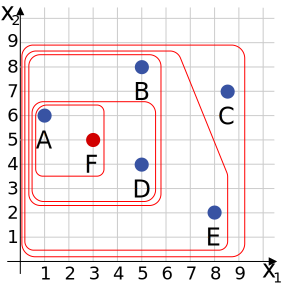
\includegraphics[width=\linewidth]{graph-3}
\caption{Graph with all the points, $F$ is the last added point}
\end{subfigure}%
\begin{subfigure}{.5\linewidth}
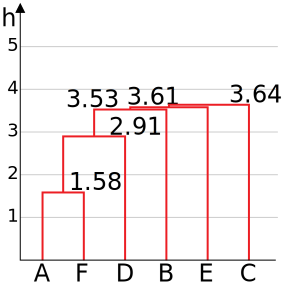
\includegraphics[width=\linewidth]{dendrogram-3}
\caption{Dendrogram}
\end{subfigure}
\caption{Situation}
\end{figure}

%TODO: We tried different scheduling (static, dynamic private) but static was the fastest one.

\hypertarget{how-to-use-the-library}{
\section{How to use the library}
\label{how-to-use-the-library}}

%    TODO: Requires C++ 20
%TODO: the data samples can have whatever dimension you want, provided that all the samples have
%the same dimension.
%    TODO: Missing specification of which compiler flags we have used (at least -O3 and
%   -march=native)
%TODO: Cache sizes?
%   TODO: Structure used in the tests to hold pi and lambda --> std::vector

We organized the implementations of the clustering algorithms into a library composed of two
main classes, namely the\\
\texttt{SequentialClustering} and the \texttt{ParallelClustering} classes.
The first, defined in the \texttt{SequentialClustering.h} header file provides the sequential
implementation of the clustering algorithm, while the second, defined in the
\texttt{ParallelClustering.h} header file, provides all the parallel implementations of the
clustering algorithm.

\hypertarget{parallel-clustering}{%
\subsection{\texttt{ParallelClustering} class}
\label{parallel-clustering}}
This class offers several utility methods and constants allowing the programmer to easily deal
with aligned memory. In particular, the \texttt{computeSseDimension} and
\texttt{computeAvxDimension} static methods allows to compute the number of \texttt{double}
elements each data sample must be compose of, taking into account also possible paddings.

However, the \texttt{cluster} static method is most important one offered by this class. It clusters
the given data samples using the specified distance computation algorithm (see
\ref{distance-computation-algorithms} for the list of available algorithms).
It is specified as a template argument so to compile only the code needed to execute the selected
algorithm.
The method allows also to specify also the number of threads to use in each of the steps that can be
parallelized, namely:
\begin{enumerate}
\item The computation of the distance between the data samples;
\item The operations needed to fix the structure of the dendrogram after a new point is
added, i.e., fixing the representative of all the points whose representative joined a
cluster containing the new data sample (the step \textit{4} of the algorithm);
\item The computation of the square roots of the distances stored in $\lambda$.
\end{enumerate}
Note that the parallelization of such steps can be enabled or disabled at compile time by using the
template parameters of the \texttt{ParallelClustering} class.

\hypertarget{par-data-samples-layout}{
\subsubsection{Data samples memory layout}
\label{par-data-samples-layout}}

The \texttt{cluster} static method allows a certain flexibility in the memory layout of the data
samples. In particular, the method accepts two main organizations:
\begin{enumerate}
\item A contiguous region of memory, where the data samples are stored one after the other.
The method accepts either an iterator iterating over that region, or directly the data
structure holding it. In this case, the \texttt{cluster} method takes care of extracting the
iterator by calling the \texttt{begin} method or, if present, the \texttt{cbegin} one;

\item A data layout organized in two levels.

The first level is merely a container that holds the data samples to cluster (or the iterators
iterating over them). This container is required to be randomly accessible, but it is not
required to be contiguous in memory.

Each element of the second level is a data structure (or an iterator iterating over it) holding a
contiguous region of memory that stores the attributes of one data sample.

For both levels, the \texttt{cluster} method accepts either the iterator over the data structure, or
the data structure itself. In this last case, the method takes care of calling the
\texttt{begin} method, or the \texttt{cbegin} one if present, to obtain an iterator iterating
over the data structure.

\end{enumerate}

\hypertarget{par-pi-lambda-layout}{
\subsubsection{\boldmath$\pi$ and \boldmath$\lambda$ memory layouts}
\label{par-pi-lambda-layout}}

The \texttt{cluster} static method allows also a certain flexibility in the memory layout of
$\pi$ and $\lambda$.

In particular, each of them can be any randomly accessible data structure, or an iterator
iterating over it.
In the former case, the method takes care of calling \texttt{begin} method, or the
\texttt{cbegin} one if present, to retrieve the random access iterator iterating over the
specified data structure.

Note that the \texttt{cluster} method assumes the data structures holding $\pi$ and
$\lambda$ to be as big as the number of data samples to cluster.

\hypertarget{distance-computation-algorithms}{
\subsubsection{Distance computation algorithms}
\label{distance-computation-algorithms}}

The \texttt{cluster} stating method allows the programmer to use different algorithms to compute
the distance between two data samples. In particular:
\begin{itemize}
\item \texttt{CLASSICAL}, which computes the Euclidean distances without using any SIMD
instruction;
\item \texttt{SSE} and \texttt{AVX}, which compute the distances using SSE and AVX
instructions respectively;
\item \texttt{SSE\textunderscore OPTIMIZED} and \texttt{AVX\textunderscore OPTIMIZED}, which
compute the distances using
SSE and AVX instructions respectively, and they keep the partial sums in the registers
instead of storing them into a variable (see
\ref{micro-optimization-partial-sum});
\item \texttt{SSE\textunderscore
OPTIMIZED\textunderscore NO\textunderscore SQUARE\textunderscore ROOT} and\\
\texttt{AVX\textunderscore OPTIMIZED\textunderscore NO\textunderscore SQUARE\textunderscore
ROOT}, which act like\\ \texttt{SSE\textunderscore OPTIMIZED} and
\texttt{AVX\textunderscore OPTIMIZED} respectively, but they compute the square of the distances,
without applying the square root operation (see \ref{micro-optimization-no-square-root}).
\end{itemize}

\hypertarget{sequential-clustering}{
\subsection{\texttt{SequentialClustering} class}
\label{sequential-clustering}}

This class provide only one method, the \texttt{cluster} static method, which executes the
sequential implementation of the clustering algorithm on the specified data samples.

\hypertarget{seq-data-samples-layout}{
\subsubsection{Data samples memory layout}
\label{seq-data-samples-layout}}

The \texttt{cluster} static method supports the same data layouts as the \texttt{cluster} method
of the parallel implementation (see \ref{par-data-samples-layout}).

In addition, if the specified data structure (or iterator) is organized in two levels, then this
method does require the first level to be randomly accessible, but it requires only the first
level to be input iterable (or to be an input iterator).

\hypertarget{seq-pi-lambda-layout}{
\subsubsection{\boldmath$\pi$ and \boldmath$\lambda$  memory layouts}
\label{seq-pi-lambda-layout}}

The \texttt{cluster} static method supports exactly the same data layouts for both $\pi$
and $\lambda$ as the \texttt{cluster} method
of the parallel implementation (see \ref{par-pi-lambda-layout}).

\hypertarget{timers}{
\subsection{\texttt{Timer} class}
\label{timer}}

If you define the \texttt{TIMERS} macro, both the sequential and parallel implementations of the
clustering algorithm will measure the time taken to execute each step of the algorithm using a
timer.

In particular, each step is measured by a different timer identified with the following identifiers:
\begin{itemize}
\item \texttt{0} measures the time taken to execute all the service operations,
like moving the iterators, or initializing the internal data structures;
\item \texttt{1} measures the time taken to initialize $\pi$ and $\lambda$;
\item \texttt{2} measures the time taken to compute the distance between the data
samples;
\item \texttt{3} measures the time taken to add to the dendrogram the new data sample;
\item \texttt{4} measures the time taken to fix the structure of the dendrogram after
a new point is added. This implies updating the representative of a data sample whenever its
current representative gets connected to a cluster containing the new point;
\item \texttt{5} measures the time taken to compute the square roots of the values in
$\lambda$. This time is measured only for the parallel implementation if the distance
computation algorithm is one of \texttt{SSE\textunderscore
OPTIMIZED\textunderscore NO\textunderscore SQUARE\textunderscore ROOT} or\\
\texttt{AVX\textunderscore OPTIMIZED\textunderscore NO\textunderscore SQUARE\textunderscore ROOT}.
\end{itemize}

Using the \texttt{print} or \texttt{printTotal} static methods of the \texttt{Timer} class you
can print to the console the times measured by each timer.


%
%
%
%
%
%
%
%
\clearpage

The sequential \texttt{cluster} function has the following signature:

To invoke the sequential clustering algorithm, the following parameters
must be passed to the \texttt{cluster} function:

\begin{itemize}

\item
\texttt{dataIterator}: a dataset iterator of generic type \texttt{D}
that must satisfy the concept \texttt{DataIterator}, defined in the
header file \texttt{Types.h};
\item
\texttt{dataSamplesCount}: the number of rows in the dataset;
\item
\texttt{dimension}: the number of columns in the dataset;
\item
\texttt{piIterator}: an iterator on the \emph{pi} data structure, of
generic type \texttt{P} satisfying the \texttt{PiIterator} concept;
\item
\texttt{lambdaIterator}: an iterator on the \emph{lambda} data
structure, of generic type \texttt{L} satisfying the
\texttt{LambdaIterator} concept;
\end{itemize}

The \texttt{cluster} function assumes that the data structures
underlying the \texttt{piIterator} and \texttt{lambdaIterator} iterators
are big enough to hold all the values.


The parallel \texttt{cluster} function has the following signature:

To invoke the parallel clustering algorithm, the following parameters
must be passed to the \texttt{cluster} function:

\begin{itemize}
\item
\texttt{dataIterator}: a dataset iterator of generic type \texttt{D}
that must satisfy the concept \texttt{ParallelDataIterator}, defined
in the header file \texttt{Types.h}. In contrary to the sequential
version, this concept requires data to be addressable through the
\texttt{{[}{]}} operator to allow concurrent data access;
\item
\texttt{distanceComputationThreadsCount}: defines the number of
threads used to compute the distances between the points. By default
it is \(0\), meaning that OpenMP will use all the available CPU
threads to perform the computation. If \texttt{S2} is false, this
value is ignored;
\item
\texttt{stage4ThreadsCount}: defines the number of threads used to
perform the stage 4 of the clustering algorithm. If \texttt{S4} is
false, this value is ignored;
\item
\texttt{squareRootThreadsCount}: defines the number of threads used to
compute the square roots of the distances. If \texttt{S5} is false, or
\texttt{C} is not \texttt{SSE\_OPTIMIZED\_NO\_SQUARE\_ROOT} nor
\texttt{AVX\_OPTIMIZED\_NO\_SQUARE\_ROOT}, then this value is ignored;
\end{itemize}

The parameters \texttt{dataSamplesCount}, \texttt{dimension},
\texttt{piIterator} and \texttt{lambdaIterator} are equivalent to the
sequential version.

Moreover, the following template parameters must be specified:

\begin{itemize}
\item
\texttt{DistanceComputers}: enumeration that defines which variant of
the parallel cluster algorithm to be used to compute the distance
between the points. Its possible values are \texttt{CLASSICAL},
\texttt{SSE}, \texttt{AVX}, \texttt{SSE\_OPTIMIZED},
\texttt{AVX\_OPTIMIZED}, \texttt{SSE\_OPTIMIZED\_NO\_SQUARE\_ROOT},
\texttt{AVX\_OPTIMIZED\_NO\_SQUARE\_ROOT}. Their meaning are described
in the previous chapter;
\item
\texttt{S2}: boolean value defaulted to \texttt{true}, indicates
whether the distance computation stage of the algorithm should be
parallelized using threads;
\item
\texttt{S4}: boolean value defaulted to \texttt{false}, indicates
whether the stage 4 of the algorithm should be parallelized using
threads;
\item
\texttt{S5}: boolean value defaulted to \texttt{false}, indicates
whether the computation of the square roots of the distances should be
parallelized using threads. Effective only if \texttt{C} is either
\texttt{SSE\_OPTIMIZED\_NO\_SQUARE\_ROOT} or
\texttt{AVX\_OPTIMIZED\_NO\_SQUARE\_ROOT}.
\end{itemize}

\end{document}
